\documentclass[a4paper]{Report}
\usepackage[titletoc]{appendix}
\usepackage{graphicx}
\graphicspath{{images/}}
\usepackage{geometry}
 \geometry{a4paper,left=3cm,top=3cm,bottom=3cm,right=3cm}

\setlength{\parindent}{1cm}
\setlength{\parskip}{0.1cm}


\begin{document}

\begin{titlepage}
    \begin{center}

\textbf{Qualifying Dissertation}
\vspace{1cm}

\textbf{\large Gamification of Software Modelling Learning}
\vspace{1cm}

Alfa Ryano Yohannis\\
ary506@york.ac.uk
\vspace{1cm}

Supervisor:\\
Dimitris Kolovos\\
Fiona Polack\\
\vspace{1cm}

Department of Computer Science\\
University of York\\
United Kingdom\\
\vspace{1cm}
\today
        
\vfill
         
\end{center}
\end{titlepage}

\tableofcontents

\chapter{Abstract}
Software modelling has a fundamental role in software engineering. However, it is perceived as relatively challenging for learners to develop the necessary abstraction skills to master the subject. On the other side, gamification is now flourishing as a popular strategy to engage learners. This research attempts to exploit gameful design as an innovative approach, used to create games that reinforce learners' mastery of software modelling by developing their abstraction skills. Our approach to gameful design brings together gamification development concepts such as the Lens of Intrinsic Skill Atoms, and pedagogical design principles from several learning theories and models. The research follows the Design Science Research Methodology and exploits Model-Driven Engineering best practices. The target outputs of this research are a modelling game design and generation framework, and a number of games produced using it. The effectiveness of the framework and its games will be evaluated using controlled experiments.

\chapter{Introduction}
This research is motivated by the growing attention towards the application of gamification in various fields \cite{kolovos2015eugenia}. Gamification itself is defined as transforming an entity to become more gameful by embedding game-associated characteristics into the entity without losing its original intended functions. The common goal of gamification is improving user’s engagement with the entity through motivating by making the entity more fun. We perceive this as an opportunity to apply gamification as well to software modelling courses. Software modelling is a subject that is seen challenging to students since it requires lots of abstraction. Thus, students who didn’t possess this kind of ability might be hindered and demotivated. Employing gamification is expected will support the students to maintain their engagement along the courses and, therefore, improve their learning outcomes. 

However, in applying the gamification, we faced a challenge that there are only several papers available that discuss the application of game characteristics in software modelling and most of them are still in the preliminary research, covering only small specific topics of software modelling. Modelling, metamodelling, and model management, the core concepts of model-driven software engineering, haven’t been covered yet.  Therefore, we believe that there is a need to extend existing gamification of software modelling works to cover those core concepts as well. The gamification itself is expected can also extend our existing approaches in teaching and learning software modelling. The purpose of this research is to study the gamification of software modelling with emphasis on (1) to what extend gamification improves the learning outcomes of software modelling learning, (2) understanding the process of how gamification improves the learning outcomes, and (3) the design of gamification of software modelling learning manifested in the form of gamification frameworks.

We explain the literature review in Section 2 and propose the research proposal in Section 3. In Section 4, we describe the preliminary results. Finally, we end this qualifying dissertation with conclusions in Section 5.


\chapter{Field Survey and Review}

Since the research of the gamification of software modelling learning is multidisciplinary, it’s best to organise the literature review categorised by the contributing fields, including the subtopics resulting from the interaction between them. So far, we have identified three major contributing fields, the software modelling itself, ludology, and pedagogy as well. They will be discussed in the following subsections and a brief review about the research methodology ends this chapter.

\section{Pedagogy}
Designing the gamification of software modelling learning cannot be separated from the field of pedagogy since the core process that will be supported by the gamification is the learning process itself. Pedagogy is a source of knowledge of how we can understand learning processes and drawn principles that will guide the design of the artefact of this research. We have selected several theories and models. They are discussed briefly in the following subsections.

\subsection{Learning Process}
When we talk about learning process, it cannot be entirely separated from the cognitive process in which knowledge is constructed through sensing, experiencing, and thinking . Therefore, we need to identify what kind of steps that students need to undergo in order for them to build certain knowledge and the Bloom’s Taxonomy provides us the six categories of cognitive process: remember, understand, apply, analyse, evaluate, and create  (Krathwohl, 2002). These categories are viewed as levels of hierarchy which upper category depends on the categories below it. As an example, learners first have to remember the underlying relevant knowledge in order to understand a new concept. The categories provide us what kind of activities that should exist in the learning process starting from the simplest to the most complex one.

Like many other models, the framework also received many critics about its empirical evidence, perceived as too rigid, and simplifying the complexity of cognitive process. Nevertheless, the revised version of the taxonomy has allowed overlapping between the categories providing certain degree of flexibility to accommodate the complexity  of cognitive process (Krathwohl, 2002). The framework itself has been proven very useful to educators in designing learning courses, objectives, and evaluation and have been used for more than 50 years across disciplines (Munzenmaier \& Rubin, 2013). 

\subsection{Motivation}
\subsection{Multimodal Learning}
\subsection{Csikszentmihalyi’s Flow Theory}
\subsection{Revised Bloom’s Taxonomy}
\subsection{Kolb’s Experiential Learning Model}
\subsection{Keller’s ARCS Motivational Learning Model}
\subsection{Fleming’s VARK Multimodal Learning Model}
\section{Ludology}
\subsection{Serious Games}
\subsection{Gamification}
\section{Software Modelling}

\subsection{Software Modelling Tools}

\subsection{Software Modelling Teaching}
We have investigated related literatures regarding the teaching and learning of software modelling.  From the literatures, we have identified lessons and categorised them into 3 groups: contents, teaching or learning practices, and tool design. We will take into account the lessons during the design process of our gamified software modelling learning since we want to develop our research upon other existing works thus have stronger foundation.   

\textbf{Contents}. Contents mean the software modelling topics and their structures. In teaching software modelling, we need to teach the core, important concepts and their relation with the contexts and applications of the outside world. The contents of software modelling learning should be:
\begin{enumerate}
\item Software modelling definition \cite{borstler2012teaching}.
\item Semantics, syntaxes, notations. Teach modelling foundations, but focus more on semantics, not only syntax \cite{borstler2012teaching}. Improve use of language, not only vocabulary \cite{bezivin2009teaching}.
\item Modelling, metamodelling, and model transformation. Focus on the core, important concepts: modelling, meta-modelling, and model transformation. Teach modelling that comprise the following topics: formal and informal models, partial and complete models, distinction between models and programs \cite{bezivin2009teaching}. Meta-modelling is given a larger portion than modelling since a model might conforms to more than one meta-mode \cite{ober2007teaching}.
\item Software modelling is engineering. Teach the engineering aspects of software modelling: understanding a domain, planning and resourcing, documentation, quality, formality, validity, optimisation \cite{paige2014bad}.
\item Contexts and practices/applications in various domains \cite{paige2014bad}. Teach the application of software modelling in various domains, success stories, code generations, model discovery, and model-driven interoperability. Make the model executable. Still the power of execution makes it much easier to understand the model \cite{bezivin2009teaching}. Convey the practical applications of modelling \cite{borstler2012teaching}.
\end{enumerate}


\textbf{Teaching and Learning Practices}. Teaching and learning practices are the principles, values, and methods in teaching or learning software modelling. The followings are them:
\begin{enumerate}
\item Modelling is the process to think abstractly about systems. Therefore, we teach modelling to make students understand the value of abstraction \cite{bezivin2009teaching}. Successful application of Model-Driven Software Development requires skills in abstract modelling \cite{whittle2013industrial}.
\item Teach with prerequisites (Paige et al., 2014). Student should have a good programming background (Bezivin et al., 2010) or has to know a little about OOP (Akayama et al., 2013).
\item Encourage students to produce “good” models, and measure the “quality”. One way is to use tools (Akayama et al., 2013).
\item Teach modelling together with programming (Börstler et al., 2012). Modelling should be developed alongside programming (Bezivin et al., 2010).
\item Learn modelling as early as possible (Bezivin et al., 2010), (Börstler et al., 2012).
\item Problem-solving first, modelling language specification and modelling tools get in the way (Paige et al., 2014).
\item Provide solutions, not answers (Paige et al., 2014).
\item Teach modelling language broadly, not deeply.(Paige et al., 2014), and 
\item Teach modelling throughout (Börstler et al., 2012). Students need to experience the whole cycle of modelling in a software engineering project so they learn to decide which development process is more appropriate (Akayama et al., 2013).
\item Refer to other disciplines or other aspects related to software modelling (Paige et al., 2014).
\item Even though code generation is essential to understand modelling (Liebel, Heldal, Steghöfer, \& Chaudron, 2015),  teach other applications (benefits) of software modelling at first. Code generation comes later (Paige et al., 2014).
\item Be careful when using analogies and physical decomposition, since they might not reflect the complexity of the system; one component might have a cross-cutting effect to other layers of the system (Paige et al., 2014). 
\item It is good to teach modelling with a standard language, such as UML (Bezivin et al., 2010), but teach modelling and meta-modelling using other modelling languages as well, not just UML. Software modelling is not a UML modelling course (Paige et al., 2014). A significant number of successful Model-driven Software Development companies build their own modeling languages and generators, suggesting a re-orientation of education away from UML notation to fundamental modeling principles (Whittle \& Hutchinson, 2012).
\item Choose a playful domain or fun problems, not serious domain (Paige et al., 2014).
\end{enumerate}


\textbf{Tool Design}. Tools design are the principles in designing software modelling tools.
\begin{enumerate}
\item Learning modelling tools is not trivial (Paige et al., 2014). 
\item Build knowledge and skills incrementally \cite{lethbridge2014teaching}.
\item Use papers, tools designed for pedagogy, or use mainstream tools (Akayama et al., 2013).
\item The usage of modelling tools is not important in the beginning, but later when modelling task becomes larger (Bezivin et al., 2010).
\item A good experience with the tool has a positive influence on the students’ view of UML and modelling in general (Liebel et al., 2015).
\item Support for tool usage greatly affects student satisfaction. Provide Tool Expert and carefully design the instructions if you are using Industry Modelling Tool (Liebel et al., 2015). For an example, Papyrus is suitable for a classroom environment given the right level of support (Liebel et al., 2015).
\item Give positive reinforcement to learners \cite{lethbridge2014teaching}.
\item The tools gives maximum opportunities for learning \cite{lethbridge2014teaching}.
\item The tool convinces learners of the value of what they learn \cite{lethbridge2014teaching}.
\item Focus on high usability \cite{lethbridge2014teaching}.
\item The tool is inexpensive \cite{lethbridge2014teaching}.
\end{enumerate}


\subsection{Abstraction in Software Modelling Teaching and Learning}
Following the last discussion, modelling and meta-modelling, and additionally model management, are the potential concepts that will be taught in the game. All the three concepts requires adequate abstraction skill; a skill that has a fundamental role in Computer Science and Software Engineering (Engels, Hausmann, Lohmann, \& Sauer, 2006; Hazzan, 2008; Kramer \& Hazzan, 2006). 
There are some available strategies in teaching abstraction. Familiarity, Similarity, Reification, Application. This strategy is proposed by White and Mitchelmore in the Math education (White \& Mitchelmore, 2010). They argued that abstraction should be developed from empirical experience, move up to abstraction, and concreting the abstraction through application. Similarly, based on their experience teaching UML, Engels et al. (Engels et al., 2006) approached abstraction through modelling according to this steps: real-word objects, object diagrams, class diagrams. The real-world objects can be described by videos or may be substituted by textual explanation, animations, or pictures. Hazzan (Hazzan, 2008) proposed three methods in teaching abstraction. First, illustrate. Lecturer uses abstraction-related words or statements in teaching. Second, reflect. For an example, lecturer and students question the impact of using certain level of abstraction or not using abstraction at all. Third, practice. Students must practice and reflect on what he do.

There are two approaches of learning software modelling which a learner may perform them simultaneously: rational approach and intuitive approach (Bobkowska, 2014). Usually at the beginning of modelling process, one uses his existing knowledge and logical reasoning to understand and develop software models, and sometimes preceded with empirical activities. However, there are situations in software modelling when his existing knowledge and methodology-based, logical reasoning are not enough to make him understand or to develop a software model. Thus, make him relies on his own intuition or both approaches interplay in dealing with complex, difficult modelling. In line with Bobkowska's statement, in building a model on the correct level of abstraction, one needs a certain intuition and skill which cannot be gain through lectures but have to be experienced through exercises (Engels et al., 2006).

\subsection{Gamified Software Modelling}
Most of the gamification studies available are dominantly relates to software engineering in a larger context or other aspects of software engineering, such as software implementation and project management, rather than software modelling in particular \cite{Pedreira2015}. Several studies that apply gamification specifically for software modelling are the works of Stikkolorum et al. \cite{Stikkolorum2014}, Ionita et al. \cite{Ionita2015}, Groenewegen et al. \cite{Groenewegen2010}, and Richardsen \cite{Richardsen2014}. These works are selected because they develop artefacts based on gamification approach, apply them to software modelling, and validate the results. 

Stikkolorum et al. \cite{Stikkolorum2014} developed a game that is intended to teach software design principles, such as cohesion, coupling, information hiding, and modularity in software design.They tried to look for a solution that provides balance between coupling and cohesion by using the toolbox to draw classes, methods, attributes, and relationships between them. They applied game elements like puzzle game, game levels, visual and audio feedbacks, progress indicator, level unlocking, choice of path, multiple solutions, scoring. For the pedagogical aspect, they mentioned Bloom’s taxonomy in their work. However, they did not explain how they integrated the taxonomy into their work. After using their game, users started to talk regarding classes, methods, and associations instead of boxes, blocks, and lines, indication unconscious learning. The challenges of their work were on determining scores because there are more than one solutions for a problem. To determine coupling, they used Coupling Between Classes (CBO). Cohesion was measured by comparing all items—attributes, methods, class name—in a class that have similar keywords. Information hiding and modularity is evaluated using general design patterns. They validate their design by conducting user test and utilise the 'think aloud' method—asking users to tell their thoughts while using the game. 

Groenewegen et al. \cite{Groenewegen2010} applied gamification to improve stakeholders' understanding of their enterprise architecture models as well as to validate them.
They employ exploring the model step by step, element by element according to the given rules technique which can provides a player a progressive user experience. Therefore, it can improve user understanding. The game proposed is more playable, more freedom to try and explore, and no explicit rewards given. For the game elements, they utilise cards, explorable board-game, and rules. 
Regardless of their claim that users can understand the model better rather than by merely looking at the model so they can give argument whether the model is valid or not based on their existing knowledge, they never clearly discussed the pedagogical aspect of their work. The challenges that they experienced during the implementation of their are preparing the game by translating implicit knowledge to explicit knowledge of the model—a gap of knowledge between the modeller and the reader, which domain knowledge is required. Lack of domain knowledge will make the model less understandable and the user cannot validate the model. For validation, they tested their work to seven respondents and then interviewing them. 

In the domain of information security modelling, Ionita et al.\cite{Ionita2015} developed a socio-technical modelling language (TREsPASS) and map them toward tangible representation. Mapping the socio-technical modelling language to the tangible model is the most challenging part of their work. The tangible representations will increase the familiarity and understandability of models, which will increase awareness, involvement, and learnability. For the game elements, they utilise familiar, tangible representation, such as Lego characters, board-game metaphor, rules. They also discussed the pedagogical aspect of their design which is based on the theory of constructionvism, cognitive load, and cognitive fit. Moreover, based on their experiment, they reported that experimental group performs better than the control group in learnability, efficiency, correctness, and satisfaction. Likewise, based on interview with experts and professionals, the respondents argued that the tangible model might be useful for less technical domain experts and different types of stakeholders to be more participative and contributive in the early stages of architecture modelling.

In the context of activity diagram learning, Richardsen  \cite{Richardsen2014} developed a game which it's behaviours are controlled through arranging UML activity diagram. Throughout his research, he found challenge that controlling game from activity diagram in Reactive Block Environment (Eclipse based) is difficult since Eclipse is difficult for a first-time user. For validation, he conducted user testing with three users. Think Aloud method was used for observation. After that, questionnaires were given and an interview was conducted. he found out There was no significant different between the traditional interactive tutorial and the game-like tutorial on their performances. However, the game-like tutorial was more engaging.
Validation In his work, he did not mention any explicit pedagogical aspect.

Based on the previous four related works, we concluded that different concepts of software modelling were addressed. However, no use of game elements that addresses abstraction regarding modelling, meta-modelling, and model transformation in particular, which mean there is an opportunity for research on that area. We also found that different specific concepts were addressed with different approaches and game elements which also challenge us to develop a more generic design in addressing software modelling learning problem. The good news is all of the works reported that the use of game and game elements has positive effect in motivating and engaging users in varying degree. Furthermore, every study has their own challenges which are a good thing to be aware of when carrying our research. The drawbacks of other works are, first, most of the them did not consider seriously about pedagogical aspect of their solution and, second,in general, their validation was weak regarding sample size and lack discussion of internal validity.


\subsection{Software Modelling Course at the University of York}

\section{Research Methodology}
The software modelling learning game design framework will be derived deductively mainly from existing related theories and research works that come from the fields of education, games, and software modelling. The resulting framework will be tested in several case studies for validation and the test results will be inputs to revise the framework. Since the outputs of the research will be design artefacts, Design Science Research Methodology \cite{peffers2007design} is selected as the research methods as it provides a comprehensive conceptual framework and activity guidelines for understanding, developing, executing, and evaluating design artefacts. We also implements Deterding's Gameful Design Steps \cite{deterding2015lens} to guide the design of the gameful aspect of the the product.

\subsection{Design Science Research Methodology}
We will employ Design Science Research Methodology \cite{peffers2007design} as the methodology to carry out the research. DSRM is selected since it provides a comprehensive conceptual framework consists of activity guidelines for understanding, developing, executing, and evaluating design artefacts. Oher reason is that it positions itself at the top level of abstraction without going into much detail of how to perform each activities, we can freely choose other more concrete research methods to carry out the activities. For examples, we can conduct literature reviews, surveys, or expert interviews to determine research problems, motivations, solutions, and objectives as well as controlled experiments to measure and evaluate the effectiveness of the artefacts. 

\begin{figure}[h]
\centering
\frame{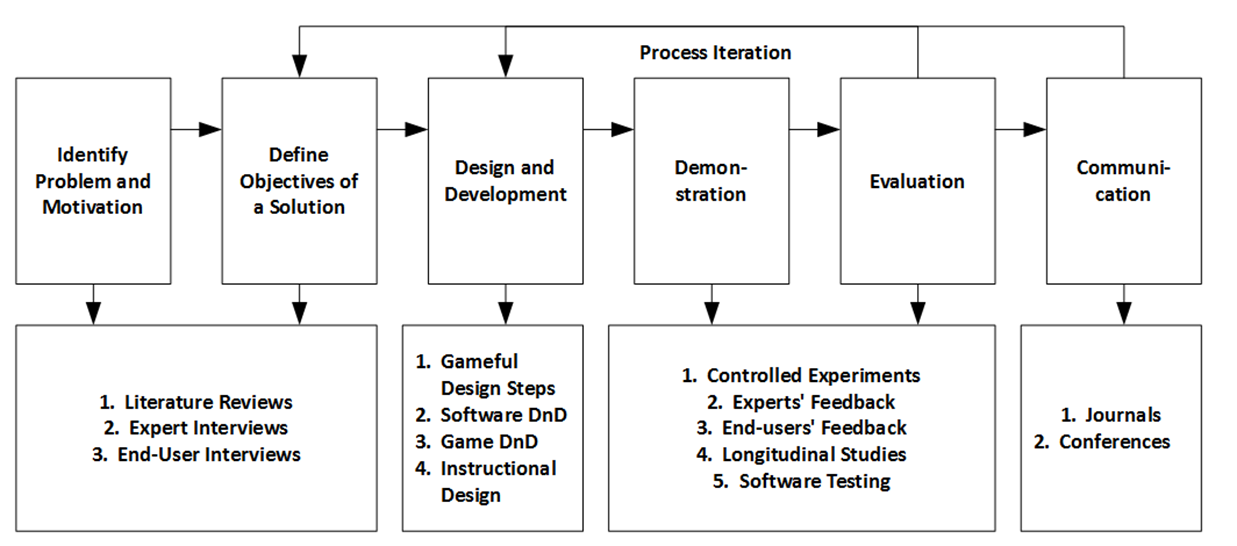
\includegraphics[width=\textwidth]{dsrm}}
\caption{Design Science Research Methodology. Adapted from Peffer et al. \cite{peffers2007design}.}
\label{fig:003}
\end{figure}

\textbf{Identify Problem and Motivation}. This research will use literature review, suggestions from experts, and surveys to identify research problems and motivations a well as to determine the solution and its objectives.

Based on the literature review, the best guesses that we have made so far regarding the challenges that student has to deal with when learning software modelling are abstracting (choosing the most relevant elements, ignoring the irrelevant ones, and determining the relationships between elements), diagramming (translating the abstraction into visual elements), and determining the algorithmic strategies (programming in the context of model management). Other challenges are no fun (the presentation of the software modelling course is not interesting) and the heavy cognitive loads when dealing with abstract objects. However, the guesses have to be confirmed yet through surveys, drawing information from students of software modelling courses in order for our problem identification to be more accurate.

As we could view the challenges as problems, this research then chooses the problem-centred initiation as its entry point since those challenges hinder learners in learning software modelling.  Grounded on the identified problems, we could decide that there is a necessity to build a tool that can support software modelling students to develop their abstraction, diagramming, and algorithmic strategy skills in a more motivating and engaging way. 

\textbf{Define Objectives of a Solution}. Based on the identified problems and motivations, we have defined our solution that is embedding gamification in the process of software modelling learning, which is expressed by the use of an artefact specifically designed with gamification and pedagogy in mind. The research objectives and outcomes are defined in section 3.2 and 3.3.

\textbf{Design and Development}. This research will employ gameful design method (Deterding, 2015) to design and develop the gamification and agile software development method to design and develop the artefact. The design and development activities are part of the iterative cycles and the products of the activities will be refined as required based the results generated from the evaluation activity.

\textbf{Demonstration and Evaluation}. The resulting artefact will be demonstrated and evaluated by applying it to several courses of software modelling. Moreover, the evaluation results will be used as feedbacks to improve the quality of artefacts and as a ground to judge the research findings.  Demonstration and evaluation activities are parts of the iterative cycles and will be performed again as required. 

\textbf{Communication}. Significant findings will be published in an academic conferences or journals for dissemination and evaluation by the related research communities.


 
\subsection{Gameful Design Method}




\chapter{Proposal}
Grounded on the literature review in Chapter 2, we base our research in these premises. First, learning software modelling is not a trivial task as it requires abstraction skills and demands high cognitive loads to deal with abstract objects and operations. Second, regardless gamification design is still an ongoing challenge \cite{Deterding2013}, it is an opportunity for research that up today there is still no work in the gamification of learning that addresses the core concepts of software modelling—modelling, metamodelling, and model transformation. Third, there is still no gamification design framework that guide the integration of game specific domain into software modelling learning. Fourth, opportunity to 

\section{Research Questions}
The main research question proposed by this research is "How can gamification improve software modelling learning?" In order to support answering the main research question, following sub research questions need to be investigated:
\begin{enumerate}
\item Which processes, aspects, principles, or components of software modelling and their teaching and learning practices would benefit from gamification?
\item What types of game elements and in what roles can deliver software modelling learning best? 
\item What kind of orchestrating framework is needed to design the interaction between software modelling and game elements to achieve software modelling gamification?
\item To what extent does gamification of software modelling improve learners' motivation, engagement, and performance?
\item To what extent do software modelling tutors benefit from software modelling game design framework?
\end{enumerate}

\section{Aim and Objectives}
In order to answer the research questions, following aim and objectives should be met. The main aim of this research is to investigate and develop a software modelling game design framework that systematically and semi-automatically drives gamification design to produce software modelling learning games. More precisely, this research aims to meet the following research objectives that are derived from the main research aim:

\begin{enumerate}
\item Perform a literature review and surveys to identify research problems, questions, and objectives as well as necessary information to carry out the selected research methods and to develop an early version of the conceptual framework and artefact as the instantiation of the framework. 
\item Develop a conceptual framework of how to design gamification of software modelling learning based on the literature review and the survey. The framework will be iteratively updated according to the results obtained from the experiments. 
\item Develop a software artefact as the instantiation of the conceptual framework to produce a gamification of software modelling learning. The gamification will be tested to respondents for evaluation and to obtain feedbacks for iterative improvement. 
\item Perform controlled experiments to measure the significance of the sofware modelling learning game in improving learning performance compared to the traditional method.
\item Perform controlled experiments to measure the productivity and maintenabilty of software modelling learning design framework in supporting tutors design and develop gamified software modelling learning. 
\end{enumerate}

\section{Research Outputs}
The potential research outputs of this research are:
\begin{enumerate}
\item Artefact. The software/application of gamification of software modelling learning.
\item Modelling Artefact. A tool for modelling the application of the gamification of software modelling learning.
\item Significance. Controlled experiments, learning outcome comparison between the gamified version and the traditional one.
\item Software Modelling Design Framework. Conceptual and software framework to perform gamification of software modelling learning.
\item Understanding. A model that explains how gamification of software modelling learning works.
This could be achieved through Learning and Game Analytics and Structural Equation Modelling studies.
\item Case Study. Report the application of theories, models, and methods used in this research.
\end{enumerate}

\chapter{Preliminary Results}

\section{Preliminary Survey}


\section{Requirements}


\section{Game Design}
Gamification has been successfully for a variety of purposes, but there is very little work on software modelling gamification. We wish to assess whether gamification is beneficial for learners of graphical software modelling languages. For each modelling language, we envision the development of a dedicated game containing game elements that will be derived from the Lens of Intrinsic Skill Atoms \cite{deterding2015lens}. The generated game will mimic a graphical modelling tool and at each level, it will require the learner to graphically construct or adapt a model to satisfy a set of requirements and constraints.
	1
The game will have levels with gradually increasing difficulty as well as variety in its challenges, to expose learners to different kinds of domains, models, and diagrams. Tutorials are planned to be embedded into the game to help learners familiarise themselves with the control system and the flow of the game. 

The game will include interim goals and intrinsic rewards to motivate learners. For software modelling, each type of modelling (e.g. object modelling, collaboration, process) will have several stories. A story will represent a specific case study to introduce learners to problems in specific domains. Every story will consist of several levels, and every level will have one or more objectives that a learner needs to accomplish to complete it. A level may also be a continuation of a previous level, giving the learner a sense of step-by-step progress to complete the domain problems. Each story and level will introduce new concepts and link them with previously introduced concepts.

A real-world problem can be very complex and time-consuming to model. Thus, the extraneous activities that are not relevant to the core concepts that are being taught should be removed. As a result, learners will be more focused on the main concepts. Thus, game elements like bite-sized actions (e.g. drag and drop), limited choices (i.e. only limited items can be dragged), and microflows (i.e. put the right element to its right place) will be implemented to facilitate learners in performing the core activities. Likewise, fuzziness will also be used to provoke learners' creativity since most of the time there is no single correct model for the problem at hand. Attractive design will also be significant to motivate learners to interact with the game. Games should be able to give immediate, glanceable, and actionable feedback to keep learners on track and monitor their progress. Interesting and varied feedback should be designed to appeal to the learners' motives. 

To reduce bias, we plan to experiment with several modelling languages (e.g. BPMN, state-charts, GSN, UML). We also plan to implement these games using web technologies so that they are easily accessible to a wide audience.

\begin{figure}[h]
\centering
\frame{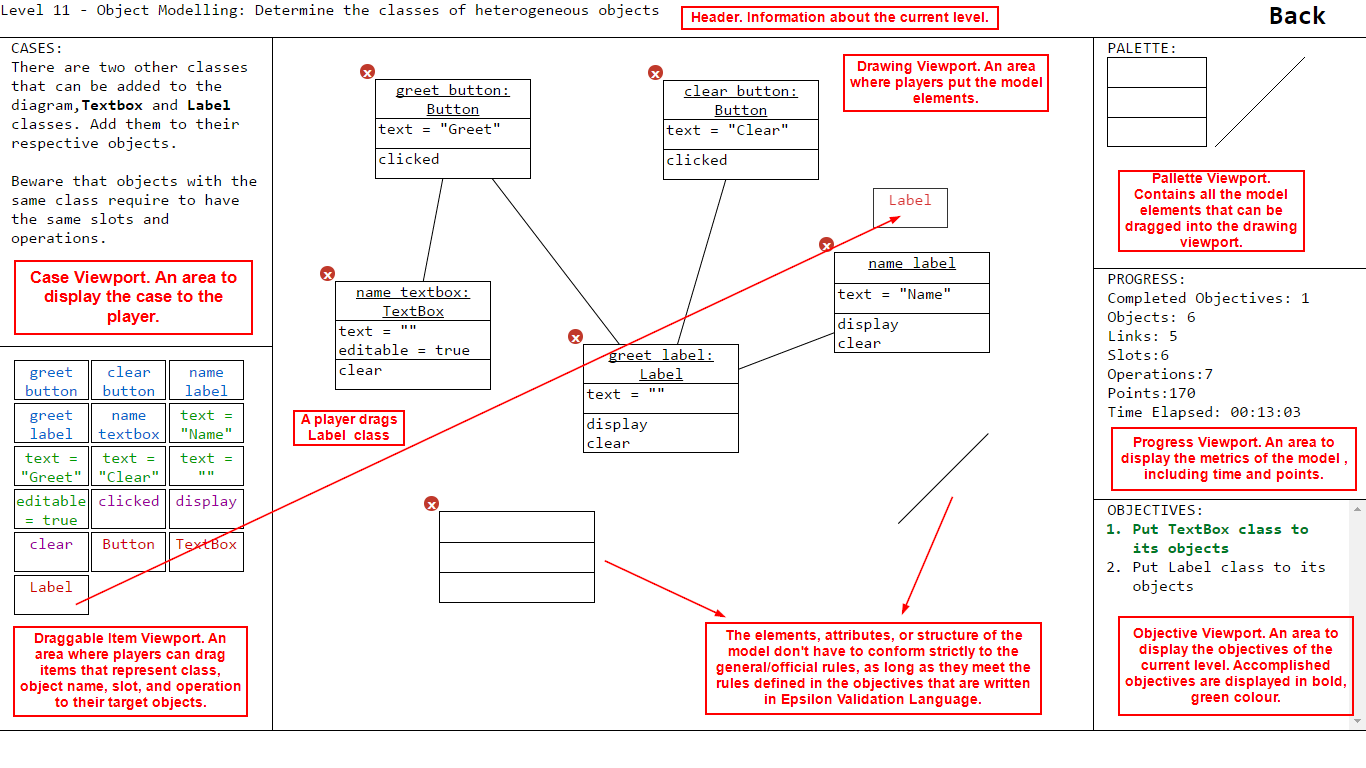
\includegraphics[width=\textwidth]{game-annotated}}
\caption{The display of the generated game.}
\label{fig:001}
\end{figure}

\section{Modelling Game Design Framework}
Instead of developing the software modelling games manually, we plan to follow a model-based approach. We will use metamodel annotations, in the spirit of Eugenia \cite{kolovos2015eugenia}, to define the graphical syntaxes of modelling languages and separate models to specify the game elements (levels, objectives, constraints, etc.) of each game. These models will be then consumed by a model-to-text transformation to produce fully-functional language-specific games. Therefore, the framework supports software modelling tutors in the design and customisation of the games at the high level of abstraction and so as to automatically build the game. So far we have implemented a metamodel for specifying game elements (flows, levels, challenges, and objectives) and a supporting Eclipse-based graphical editor (Fig. \ref{fig:002}), and a prototype game (Fig. \ref{fig:001}) for object diagrams. 

\begin{figure}[h]
\centering
\frame{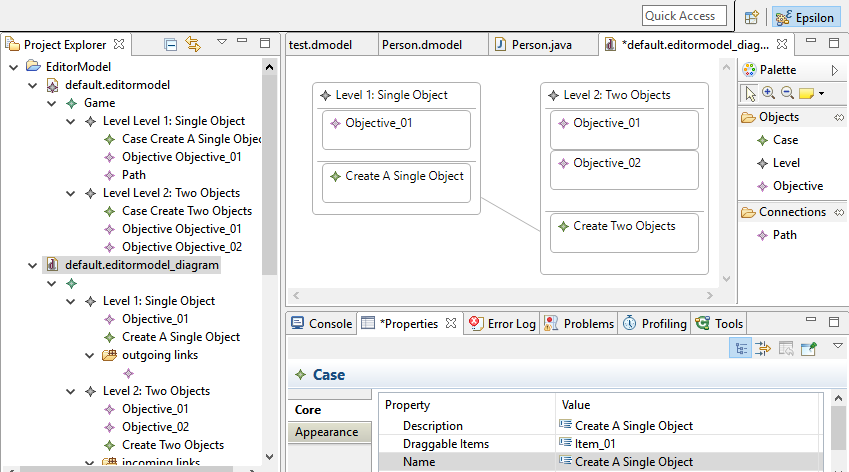
\includegraphics[width=\textwidth]{editor}}
\caption{Graphical editor for the game specification DSL.}
\label{fig:002}
\end{figure}

\addcontentsline{toc}{chapter}{Bibliography}
\bibliographystyle{IEEEtran}
\bibliography{references}

\begin{appendices}

\chapter{Research Plan}
The planned research schedule can be found in Table 1. In three years, this work plans to have five times iteration of Design-Develop-Demonstration-Evaluation, with two of them will be carry out in Indonesia and the rest of them in York.

\begin {table}[h]
\caption {Research Timetable} 
\end{table}
\begin{figure}[h]
\centering
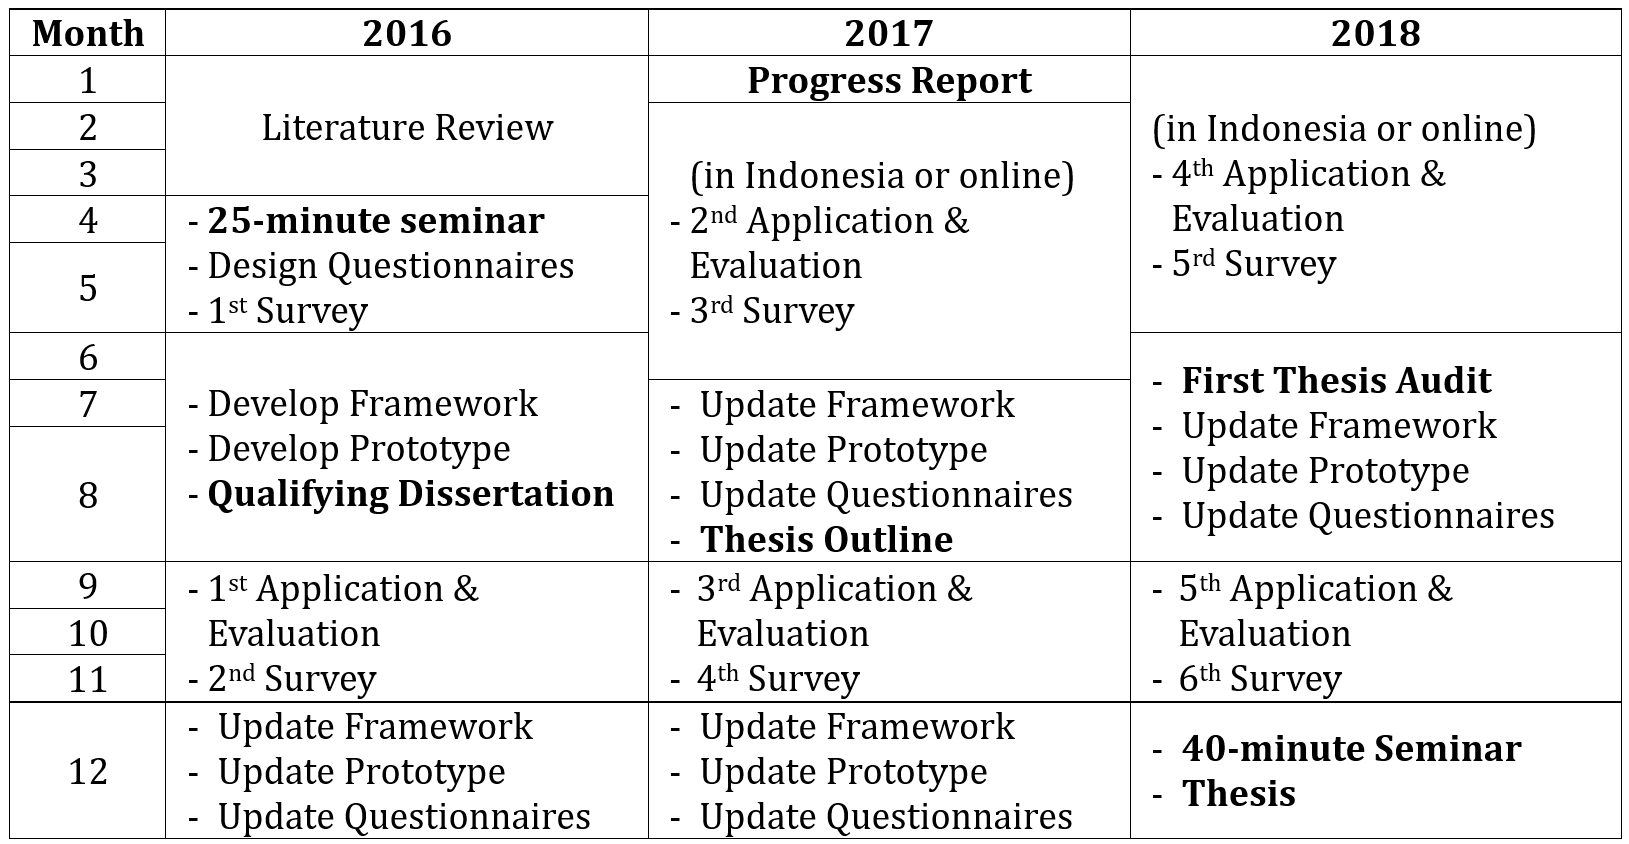
\includegraphics[width=\textwidth]{timetable}
\end{figure}

\chapter{Publications}
This research has been published in the following conferences or journals: 
\begin{enumerate}
  \item  A. Yohannis, “Gamification of software modelling,” in the ACM/IEEE 19th International Con-
ference on Model Driven Engineering Languages and Systems (MODELS 2016) Doctoral Sym-
posium. CEUR, 2016 \cite{Yohannis2016}.
\end{enumerate}

\end{appendices}

\end{document}
